\documentclass{standalone}
\usepackage{ tikz }
\usepackage{ xparse }
\usepackage{../../../macros}
\usetikzlibrary{shapes}

\begin{document}
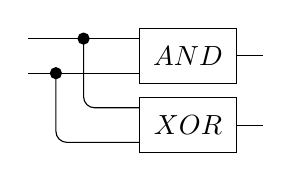
\begin{tikzpicture}[yscale=-1,x=1em,y=1.25em]
        
    \draw (0,0) -- (4,0);
    \draw (0,1) -- (4,1);
    \filldraw (1,1) circle (2pt);
    \filldraw (2,0) circle (2pt);
    \draw [rounded corners] (1,1) -- (1,3) -- (4,3);
    \draw [rounded corners] (2,0) -- (2,2) -- (4,2);

    \node [draw, minimum width=3.5em, minimum height=2em, anchor=west] at (4,0.5) {$AND$};
    \node [draw, minimum width=3.5em, minimum height=2em, anchor=west] at (4,2.5) {$XOR$};

    \draw (7.5, 0.5) -- (8.5,0.5);
    \draw (7.5, 2.5) -- (8.5,2.5);

\end{tikzpicture}
\end{document}